\documentclass{standalone}
\usepackage{graphicx}	
\usepackage{amssymb, amsmath}
\usepackage{color}

\usepackage{tikz}
\usetikzlibrary{intersections, backgrounds}

\definecolor{light}{RGB}{220, 188, 188}
\definecolor{mid}{RGB}{185, 124, 124}
\definecolor{dark}{RGB}{143, 39, 39}
\definecolor{highlight}{RGB}{180, 31, 180}
\definecolor{gray10}{gray}{0.1}
\definecolor{gray20}{gray}{0.2}
\definecolor{gray30}{gray}{0.3}
\definecolor{gray40}{gray}{0.4}
\definecolor{gray60}{gray}{0.6}
\definecolor{gray70}{gray}{0.7}
\definecolor{gray80}{gray}{0.8}
\definecolor{gray90}{gray}{0.9}
\definecolor{gray95}{gray}{0.95}

\newcommand*{\offset}{0.025}

\newcommand{\ev}[1]{\ensuremath{\,\, #1  \hspace{-0.85em}
  \mbox{\raisebox{-0.2em}{\scalebox{1.5}{$\Box$}}} } }

\begin{document}

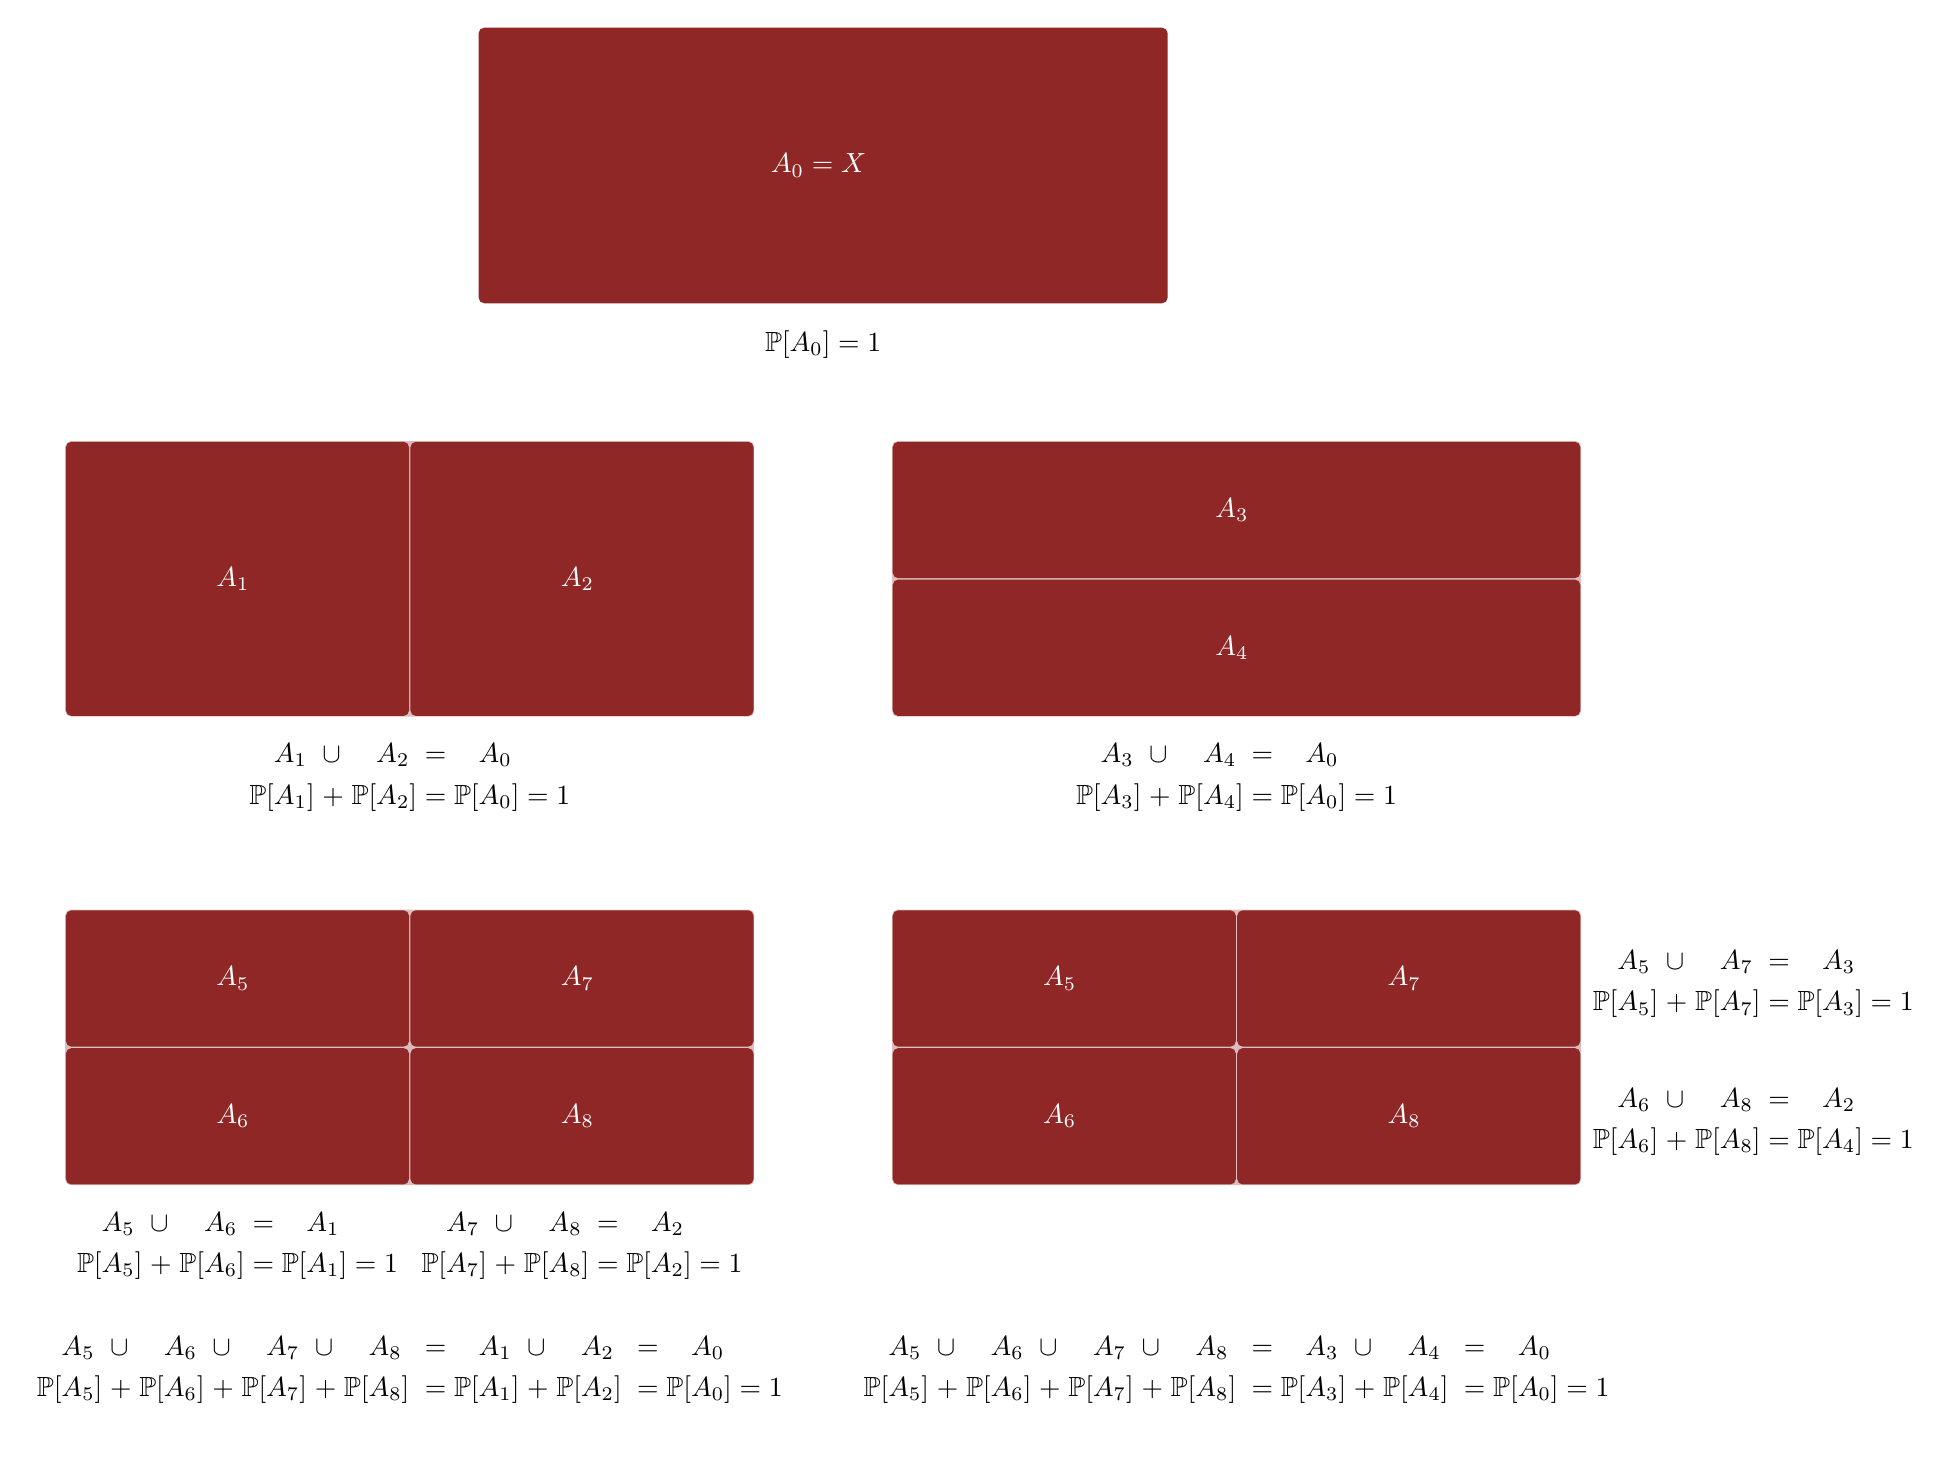
\begin{tikzpicture}[scale=0.35, thick]
  \fill [rounded corners=2pt, fill=dark, text=white] (0, 0) rectangle +(25, 10) 
  node[midway, align=center] { $A_{0} = X$ };
  
  \node[] at (12.5, -1.5) { $\mathbb{P} [ A_{0} ] = 1$ };
  
  \fill [rounded corners=2pt, fill=light, text=white] (-15, -15) rectangle +(25, 10);
  \fill [rounded corners=2pt, fill=dark, text=white] (-15 + \offset, -15 + \offset) 
    rectangle +(12.5 - 2 * \offset, 10 - 2 * \offset)
  node[midway, align=center] { $A_{1}$ };
  \fill [rounded corners=2pt, fill=dark, text=white] (-15 + 12.5 + \offset, -15 + \offset) 
    rectangle +(12.5 - 2 * \offset, 10 - 2 * \offset)
  node[midway, align=center] { $A_{2}$ };

  \node[] at (-15 + 12.5, -17) {
    \parbox{2cm}{
	  \begin{alignat*}{9}
	    &A_{1}& &\cup& &A_{2} &=& &A_{0}& \\ 
        \mathbb{P} [&A_{1}&] \;&+&\; \mathbb{P} [&A_{2}] \;&=&\; \mathbb{P} [&A_{0}&] = 1
      \end{alignat*}
    }
  };                     
                                  
  \fill [rounded corners=2pt, fill=light, text=white] (15, -15) rectangle +(25, 10);
  \fill [rounded corners=2pt, fill=dark, text=white] (15 + \offset, -15 + \offset) 
    rectangle +(25 - 2 * \offset, 5 - 2 * \offset)
  node[midway, align=center] { $A_{4}$ };
  \fill [rounded corners=2pt, fill=dark, text=white] (15 + \offset, -10 + \offset) 
    rectangle +(25 - 2 * \offset, 5 - 2 * \offset)
  node[midway, align=center] { $A_{3}$ };

  \node[] at (15 + 12.5, -17) {
    \parbox{2cm}{
	  \begin{alignat*}{9}
	    &A_{3}& &\cup& &A_{4} &=& &A_{0}& \\ 
        \mathbb{P} [&A_{3}&] \;&+&\; \mathbb{P} [&A_{4}] \;&=&\; \mathbb{P} [&A_{0}&] = 1
      \end{alignat*}
    }
  };  

  \fill [rounded corners=2pt, fill=light, text=white] (-15, -32) rectangle +(25, 10);
  \fill [rounded corners=2pt, fill=dark, text=white] (-15 + \offset, -32 + \offset) 
    rectangle +(12.5 - 2 * \offset, 5 - 2 * \offset)
  node[midway, align=center] { $A_{6}$ };
  \fill [rounded corners=2pt, fill=dark, text=white] (-15 + \offset, -27 + \offset) 
    rectangle +(12.5 - 2 * \offset, 5 - 2 * \offset)
  node[midway, align=center] { $A_{5}$ };
  \fill [rounded corners=2pt, fill=dark, text=white] (-15 + 12.5 + \offset, -32 + \offset) 
    rectangle +(12.5 - 2 * \offset, 5 - 2 * \offset)
  node[midway, align=center] { $A_{8}$ };
  \fill [rounded corners=2pt, fill=dark, text=white] (-15 + 12.5 + \offset, -27 + \offset) 
    rectangle +(12.5 - 2 * \offset, 5 - 2 * \offset)
  node[midway, align=center] { $A_{7}$ };

  \node[] at (-15 + 6.25, -34) {
    \parbox{2cm}{
	  \begin{alignat*}{9}
	    &A_{5}& &\cup& &A_{6} &=& &A_{1}& \\ 
        \mathbb{P} [&A_{5}&] \;&+&\; \mathbb{P} [&A_{6}] \;&=&\; \mathbb{P} [&A_{1}&] = 1
      \end{alignat*}
    }
  };  

  \node[] at (-15 + 18.75, -34) {
    \parbox{2cm}{
	  \begin{alignat*}{9}
	    &A_{7}& &\cup& &A_{8} &=& &A_{2}& \\ 
        \mathbb{P} [&A_{7}&] \;&+&\; \mathbb{P} [&A_{8}] \;&=&\; \mathbb{P} [&A_{2}&] = 1
      \end{alignat*}
    }
  };  

  \node[] at (-15 + 12.5, -38.5) {
	\parbox{2cm}{
	  \begin{alignat*}{34}
		&A_{5}& &\cup& &A_{6}& &\cup& &A_{7}& &\cup& &A_{8}& &=&
		&A_{1}& &\cup& &A_{2}& &=& &A_{0}& \\ 
		\mathbb{P} [&A_{5}&] \;&+&\; \mathbb{P} [&A_{6}&] \;&+&\;
		\mathbb{P} [&A_{7}&] \;&+&\; \mathbb{P} [&A_{8}&] \;&=&\;
		\mathbb{P} [&A_{1}&] \;&+&\; \mathbb{P} [&A_{2}&]
		\;&=&\; \mathbb{P} [&A_{0}&] = 1
	  \end{alignat*}
	}
  };
                                          
  \fill [rounded corners=2pt, fill=light, text=white] (15, -32) rectangle +(25, 10);
  \fill [rounded corners=2pt, fill=dark, text=white] (15 + \offset, -32 + \offset) 
    rectangle +(12.5 - 2 * \offset, 5 - 2 * \offset)
  node[midway, align=center] { $A_{6}$ };
  \fill [rounded corners=2pt, fill=dark, text=white] (15 + \offset, -27 + \offset) 
    rectangle +(12.5 - 2 * \offset, 5 - 2 * \offset)
  node[midway, align=center] { $A_{5}$ };
  \fill [rounded corners=2pt, fill=dark, text=white] (15 + 12.5 + \offset, -32 + \offset) 
    rectangle +(12.5 - 2 * \offset, 5 - 2 * \offset)
  node[midway, align=center] { $A_{8}$ };
  \fill [rounded corners=2pt, fill=dark, text=white] (15 + 12.5 + \offset, -27 + \offset) 
    rectangle +(12.5 - 2 * \offset, 5 - 2 * \offset)
  node[midway, align=center] { $A_{7}$ };

  \node[] at (40 + 6.25, -24.5) {
    \parbox{2cm}{
	  \begin{alignat*}{9}
	    &A_{5}& &\cup& &A_{7} &=& &A_{3}& \\ 
        \mathbb{P} [&A_{5}&] \;&+&\; \mathbb{P} [&A_{7}] \;&=&\; \mathbb{P} [&A_{3}&] = 1
      \end{alignat*}
    }
  };  
  
  \node[] at (40 + 6.25, -29.5) {
    \parbox{2cm}{
	  \begin{alignat*}{9}
	    &A_{6}& &\cup& &A_{8} &=& &A_{2}& \\ 
        \mathbb{P} [&A_{6}&] \;&+&\; \mathbb{P} [&A_{8}] \;&=&\; \mathbb{P} [&A_{4}&] = 1
      \end{alignat*}
    }
  };  

  \node[] at (15 + 12.5, -38.5) {
	\parbox{2cm}{
	  \begin{alignat*}{34}
		&A_{5}& &\cup& &A_{6}& &\cup& &A_{7}& &\cup& &A_{8}& &=&
		&A_{3}& &\cup& &A_{4}& &=& &A_{0}& \\ 
		\mathbb{P} [&A_{5}&] \;&+&\; \mathbb{P} [&A_{6}&] \;&+&\;
		\mathbb{P} [&A_{7}&] \;&+&\; \mathbb{P} [&A_{8}&] \;&=&\;
		\mathbb{P} [&A_{3}&] \;&+&\; \mathbb{P} [&A_{4}&]
		\;&=&\; \mathbb{P} [&A_{0}&] = 1
	  \end{alignat*}
	}
  };
  
\end{tikzpicture}

\end{document}  